\chapter{Hands-On: DDD Sample Application}
\section{Import der DDD Applikation in die IDE}
\begin{longtable}{| p{5cm} | p{11cm} |}
\hline
Die Vorlage Applikation kann in Eclipse als bestehendes Maven Projek importiert werden.
&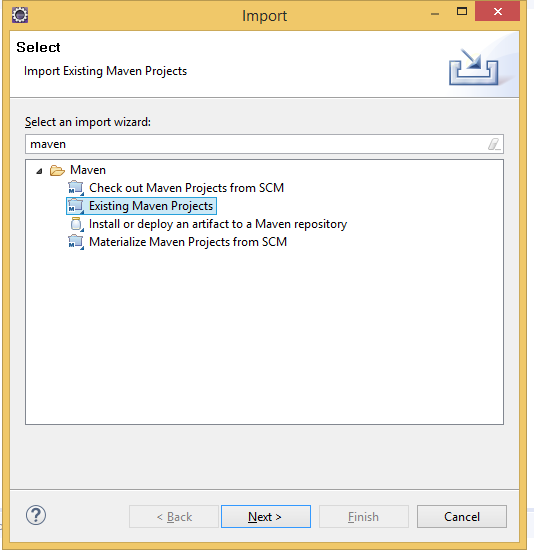
\includegraphics[width=0.65\columnwidth, valign=T]{images/ddd_basic/1.png}
 \\ \hline
Im Projektverzeichnis die pom.xml Datei auswählen.
&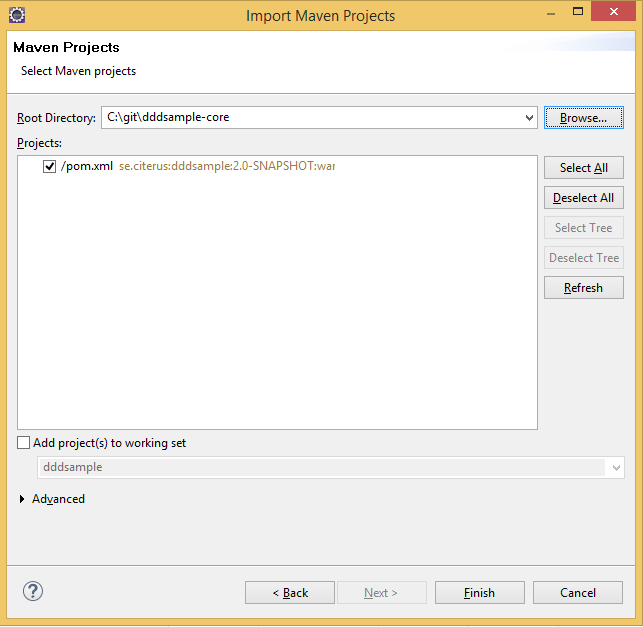
\includegraphics[width=0.65\columnwidth, valign=T]{images/ddd_basic/2.png}
 \\ \hline
Die Swisscom PaaS Cloud arbeitet mit Cloud Foundry. Das Cloud Foundry Plugin für Eclipse kann über den MarketPlace installiert werden.
&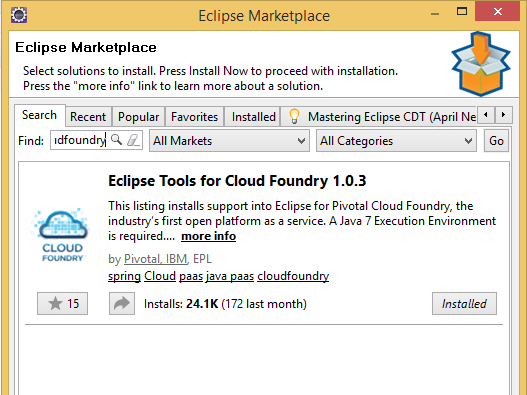
\includegraphics[width=0.65\columnwidth, valign=T]{images/ddd_basic/3.png}
 \\ \hline 
Nun müssen die Maven Dependencies geladen werden.
&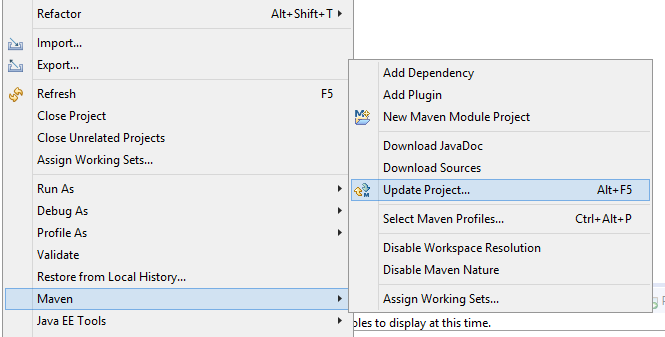
\includegraphics[width=0.65\columnwidth, valign=T]{images/ddd_basic/4.png}
 \\ \hline
Jetzt kann der Build-Prozess gestartet werden.
&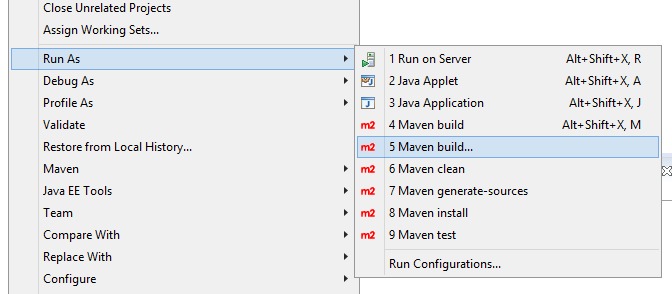
\includegraphics[width=0.65\columnwidth, valign=T]{images/ddd_basic/5.png}
\\ \hline 
\end{longtable}
\newpage
\section{Deployment in die Swisscom PaaS Cloud}
Bevor die Applikation in die Cloud gepusht werden kann muss ein Space angelegt werden. Danach kann die ddd-App in diesen Space deployed werden.
\begin{longtable}{| p{5cm} | p{11cm} |}
\hline
Eine Organisation kann mehrere Spaces enthalten. Eine Applikation wird in einen Space deployed. Wir erstellen deshalb eine neue Org.
&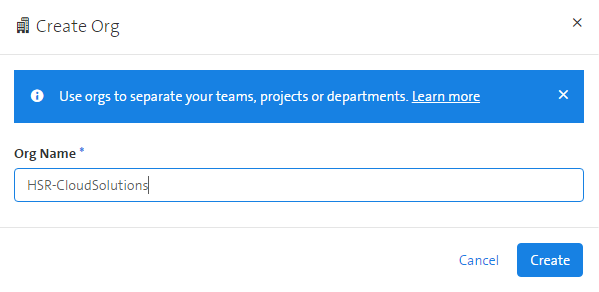
\includegraphics[width=0.65\columnwidth, valign=T]{images/swisscom_create_space/1.png}
 \\ \hline
Als Space Name wählen wir ddd (Name der App).
&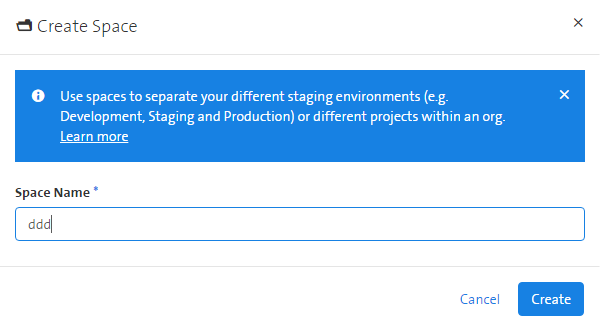
\includegraphics[width=0.65\columnwidth, valign=T]{images/swisscom_create_space/2.png}
 \\ \hline
In Eclipse muss ein neuer Server erfasst werden. Anstatt Tomcat verwenden wir nun einen Cloud Foundry Server
&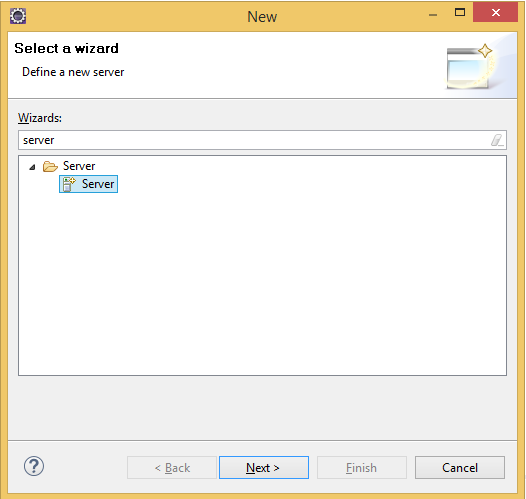
\includegraphics[width=0.65\columnwidth, valign=T]{images/ddd_cloud_deployment/1.png}
 \\ \hline 
Durch das zuvor im Marketplace installierte Plugin kann nun ein Cloud Foundry Server ausgewählt werden.
&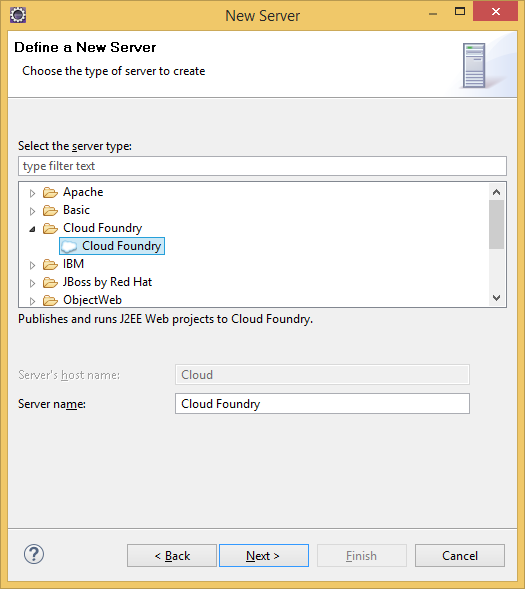
\includegraphics[width=0.65\columnwidth, valign=T]{images/ddd_cloud_deployment/2.png}
 \\ \hline
Die Logindaten des Swisscom Application Cloud Accounts müssen hier hinterlegt werden. Die URL \glqq https://api.lyra-836.appcloud.swisscom.com\grqq  muss erfasst werden.
&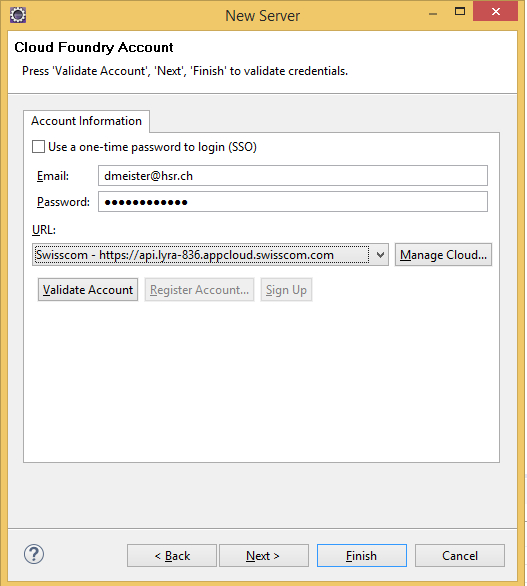
\includegraphics[width=0.65\columnwidth, valign=T]{images/ddd_cloud_deployment/3.png}
 \\ \hline
Die zuvor erstellte Org und Space sollten nun erscheinen. Den gewünschten Space auswählen um fortzufahren.
&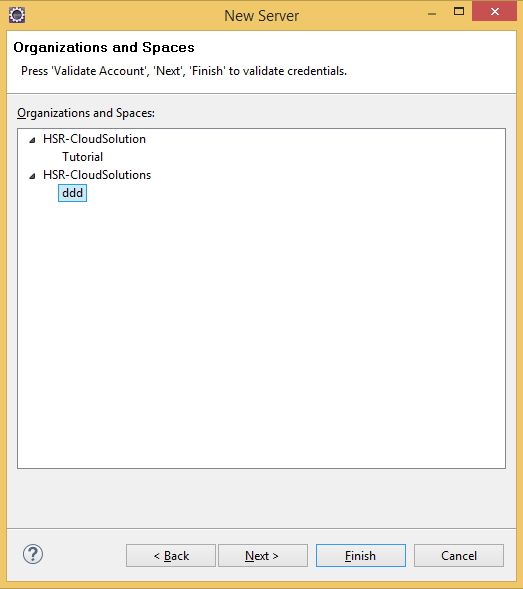
\includegraphics[width=0.65\columnwidth, valign=T]{images/ddd_cloud_deployment/4.png}
 \\ \hline 
Den App Namen kann man belassen oder falls gewünscht anpassen.
&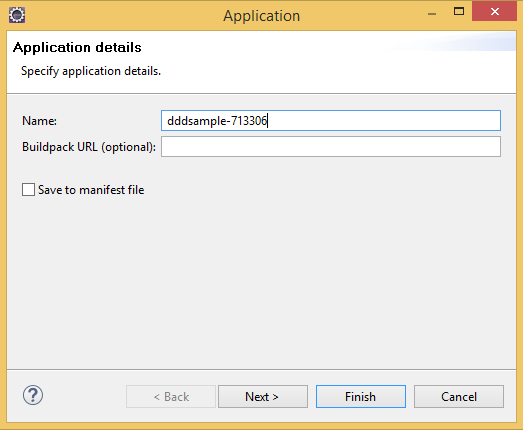
\includegraphics[width=0.65\columnwidth, valign=T]{images/ddd_cloud_deployment/5.png}
 \\ \hline
Falls benötigt kann das Memory Limit erhöht werden.
&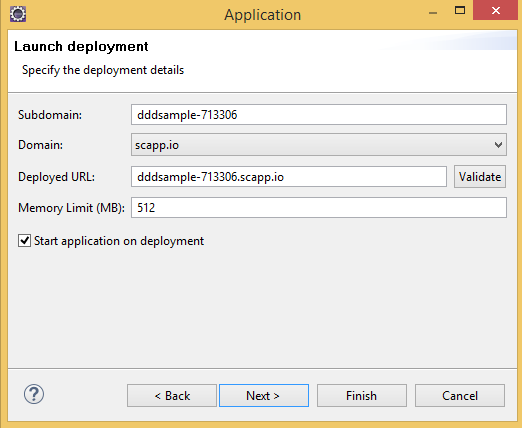
\includegraphics[width=0.65\columnwidth, valign=T]{images/ddd_cloud_deployment/6.png}
 \\ \hline
Nun startet der Deployment Prozess, nach kurzer Zeit ist er erfolgreich abgeschlossen.
&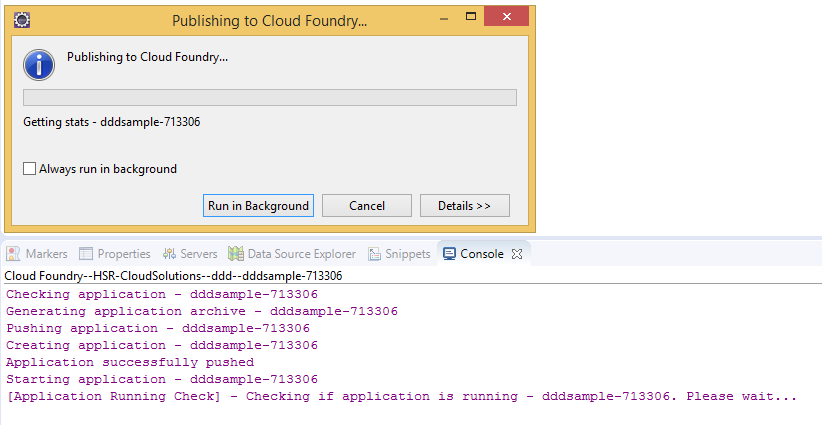
\includegraphics[width=0.65\columnwidth, valign=T]{images/ddd_cloud_deployment/7.png}
 \\ \hline
Auf der Application Cloud Console erscheint nun die laufende App.
&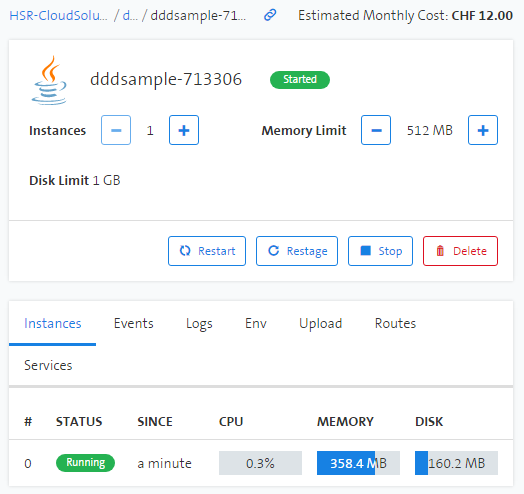
\includegraphics[width=0.65\columnwidth, valign=T]{images/ddd_cloud_deployment/8.png}
 \\ \hline
\end{longtable}
\section{Fazit}
Der grundlegende Teil dieser Aufgabe war mit der Swisscom Application Cloud sehr angenehm zu lösen. Durch die Online-Dokumentation wird man gut durch das Deployment durchgeführt. Die Applikation selbst, respektive der Code musste nicht angepasst werden. 

Anfangs hatten wir der Ausführung von gewissen Funktionen. Es stellte sich schnell heraus, dass wir vergessen haben, die Maven Dependencies zu laden und das Projekt zu builden.
\chapter{Hands-On: Erweiterung um relationale Datenbank}
Die DDD Sample App arbeitet standardmässig mit HyperSQL DB (HSQLDB). Dies ist in der Datei jdbc.properties unter /src/main/resources ersichtlich. 

Die Swisscom Application Cloud bietet keinen MySQL Service. Stattdessen wird MariaDB als vertreter relationaler Datenbank angeboten. 

\begin{longtable}{| p{5cm} | p{11cm} |}
\hline
MariaDB muss auf dem zuvor erstellten Space (ddd) hinzugefügt werden. Für diese Aufgabe reicht die kleinste Variante mit 1GB Storage und 10 Connections.
&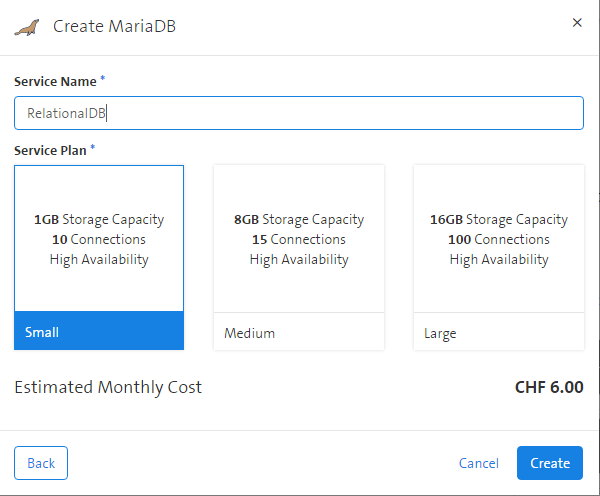
\includegraphics[width=0.65\columnwidth, valign=T]{images/mariadb/1.png}
 \\ \hline
Sobald erstellt, müssen im Reiter \glqq Serivce Keys \grqq noch Zugriffsschlüssel erstellt werden. Diese müssen dann in der verwendeten App zur Authentifizierung hinterlegt werden.
&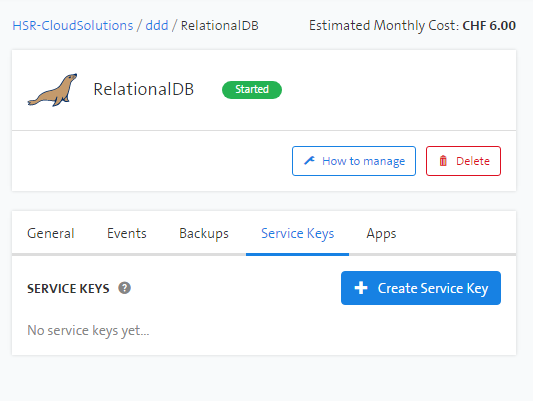
\includegraphics[width=0.65\columnwidth, valign=T]{images/mariadb/2.png}
 \\ \hline
Den Keys kann ein beliebiger Name hinterlegt werden.
&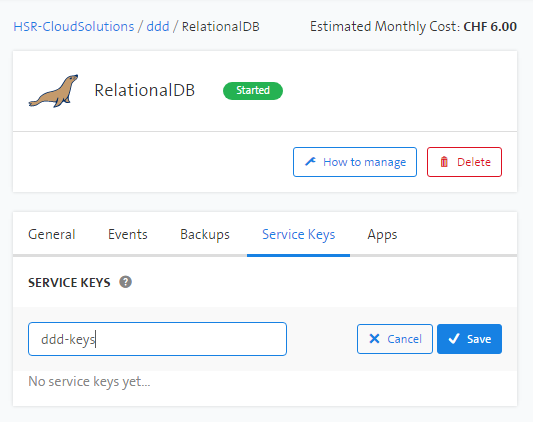
\includegraphics[width=0.65\columnwidth, valign=T]{images/mariadb/3.png}
 \\ \hline 
Die benötigten Informationen liegen nun im JSON Format da. Die private IPv4 Addresse im host-Feld verrät, dass ein externer Zugriff ausserhalb der Swisscom Application Cloud nicht möglich ist. Sowohl Username und Passwort sind ein zufällig generierter String.
&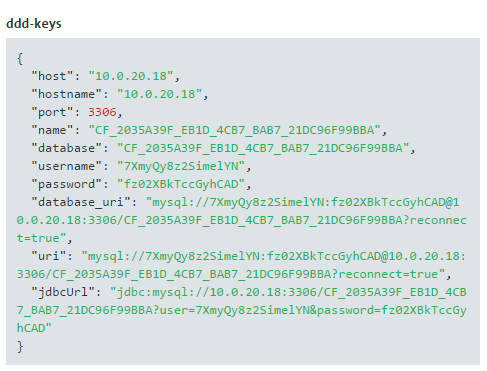
\includegraphics[width=0.65\columnwidth, valign=T]{images/mariadb/4.png}
 \\ \hline
Der bestehenden App kann nun der zuvor erstellte DB Service gebunden werden.
&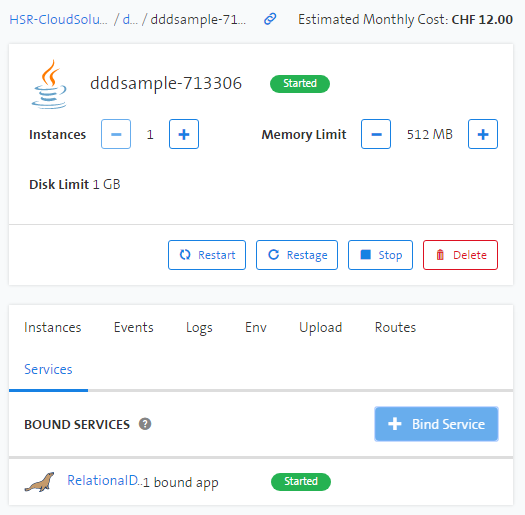
\includegraphics[width=0.65\columnwidth, valign=T]{images/mariadb/5.png}
\\ \hline 
Wir benötigen für die App nun die MariaDB Dependencies, welche wir einfach mit Maven hinzufügen können. Wir verwenden die als funktionierend empfohlene Version 1.1.7.
&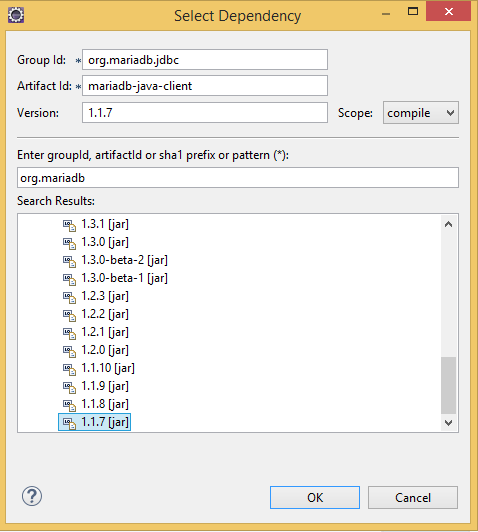
\includegraphics[width=0.65\columnwidth, valign=T]{images/mariadb/6.png}
\\ \hline 
Damit die Änderungen in der Datenbank auch nach dem Neustart persistent sind, müssen wir eine Anpassung der Konfiguration im File hibernate.properties vornehmen. Im Feld hibernate.hbm2ddl.auto müssen wir die Einstellung von \glqq create drop\grqq (nicht persistent) nach \glqq update\grqq ändern. 
&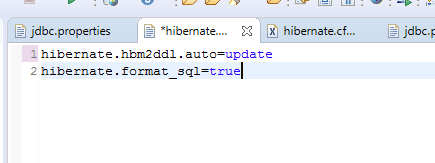
\includegraphics[width=0.65\columnwidth, valign=T]{images/mariadb/7.png}
\\ \hline 
\end{longtable}
Die Änderungen müssen nun mit Maven Update, resp. Maven Build angepasst und neu gepusht werden.

\section{Security Überlegungen}
Die Datenbankservices sind bei Swisscom nur über IP Adressen aus dem privaten Adressbereich erreichbar. Dies lässt schliessen, dass Swisscom selbst in ihrem Datacenter die Datenbanken hostet. Eine direkte Anbindung der Datenbank ausserhalb der Swisscom App Cloud ist daher nicht möglich. 

Die Zugriffe zur Datenbank sind mittels zufallsgenerierten Strings für Username und Passworte authentisiert. Eine TLS verschlüsselte Verbindung zwischen App und Datenbank wäre ebenfalls wünschenswert und im Falle eines Zugriffs aus dem Internet (hier nicht der Fall) zwingend notwendig. Wir haben leider keine Informationen betreffend Verschlüsselung der Verbindungen gefunden, und ein Sniffen des Netzwerkverkehrs ist für uns leider nicht ohne weiteres Möglich. 